\def\QRCODE{TB_image_TUT.IMG.image_characterization_pythonqrcode.png}
\def\QRPAGE{http://www.iptutorials.science/tree/master/TB_image/TUT.IMG.image_characterization/python}
\pcorrectionsection{Python correction}

\begin{python}
import matplotlib.pyplot as plt
import numpy as np
from scipy import ndimage
from scipy import signal
from scipy import misc
from scipy import spatial
from skimage import measure
\end{python}


\subsection{Perimeters}
The convolution is used here as an easy way of getting the borders of the object in one direction, i.e. counting the number of intercepts. This method is efficient because, for one given direction, a high number of lines are considered. Keep in mind that only 4 orientations are used in the proposed code.

\begin{python}
def countIntercepts(I, h):
    B = np.abs( signal.convolve2d(I, h, mode='same'));
    n = np.sum(B) / 2;
    return n;

def perimCrofton(I):
    """
    Approximate the Crofton perimeter with 4 directions
    I is the input binary image
    return the perimeter, float value
    """
    # defines an orientation
    h = np.array([[-1, 1]]);
    n1 = countIntercepts(I, h);
    
    n2 = countIntercepts(I, h.transpose());
    
    h = np.array([[1, 0], [0, -1]]);
    n3 = countIntercepts(I, h.transpose());
    
    h = np.array([[0, 1], [-1, 0]]);
    n4 = countIntercepts(I, h.transpose());
    
    perim_Crofton = np.pi/4 * (n1+n2+ 1/np.sqrt(2)*(n3+n4));
    return perim_Crofton;
\end{python}

\begin{sh}
Crofton perimeter:  1305.50015965
Classical perimeter in N4:  1374.19509294
Classical perimeter in N8:  1642.82842712
\end{sh}

\subsection{Feret diameter}
The code consists in rotating the image and evaluating the projected diameter. The rotation function can interpolate the pixel, the nearest method is thus required. The function \pinline{np.max} directly performs the projection in one direction.
\begin{python}
def feretDiameter(I):
    """
    I: input binary image
    Returns min, max and mean Feret diameter, which is the length of the 
    projected object in one direction
    """
    diameter = [];
    for angle in range(180):
        I2 = ndimage.interpolation.rotate(I, angle, mode='nearest');
        I3 = I2.max(axis=0);
        diameter.append(np.sum(I3 > 0));
    
    return np.min(diameter), np.max(diameter), np.mean(diameter);
\end{python}

For the camel image \cite{KimiaDB}, the Feret diameters are:
\begin{sh}
min, Max, average Feret diameters:  182 325 266.05
\end{sh}

\subsection{Circularity}
For a disk, the perimeter is $\pi\cdot D$ and the surface is $\pi\cdot\frac{D^2}{4}$, which shows that the circularity criterion has value 1 for a disk.

In order to generate a binary image containing a disk, one simple way is to use the formula:
$(x-x_0)^2+(y-y_0)^2\leq R^2$. The efficient way to do this is to use \pinline{np.meshgrid}.

\begin{python}
def disk(t, r):
    """
    Generates a binary array representing a disk, centered, of radius r
    an array of size [2t,2t] is generated
    """
    x = np.arange(-t, t, 1);
    X,Y = np.meshgrid(x, x);
    I = (X**2 + Y**2)<= r**2;
    return I;
\end{python}

The circularity uses the perimeters as evaluated earlier.
\begin{python}
def circularity(I):
    """
    Circularity criterion
    4*pi*A/P**2
    returns crofton and classic
    """
    P = perimCrofton(I);
    print("Perimeter by crofton: ", P)
    A = np.sum(I);
    C = np.pi*4*A/P**2;
    
    p = measure.perimeter(I, neighbourhood=4);
    print("Usual perimeter: ", p)
    c = np.pi*4*A/p**2;
    return C, c;
\end{python}
This gives for the camel image:
\begin{sh}
Perimeter by crofton:  2514.43300853
Usual perimeter:  2649.36074863
circularity by crofton:  0.999019146137
circularity usual  0.89985338478
\end{sh}

\subsection{Convexity}
The convex hull is computed with the \pinline{scipy.spatial} tools. The following function plots the result. Notice that the coordinates of an image and the coordinates of an array are different, and one has to flip the image array in order to display both data in the same figure.
\begin{python}
def convexity(I):
    """
    Evaluates the convexity criterion
    I is a binary image (np array)
    return convexity
    """
    # be careful that coordinates between images and arrays are inversed
    # thus, image is flipped before extracting points coordinates
    points = np.transpose(np.where(np.flip(I,0)));
    hull = spatial.ConvexHull(points);
    A = np.sum(I);
    Ah = hull.volume;
    
    plt.figure()
    for simplex in hull.simplices:
        plt.plot(points[simplex, 1], points[simplex, 0], 'k-')
    plt.axis('equal')
    plt.show()
    return A/Ah;
\end{python}
This criterion is between 0 and 1. This is illustrated in Fig.\ref{fig:tutorial:characterization:python:convhull}.
\begin{sh}
convexity of Camel:  0.644014426566
\end{sh}

\begin{figure}
 \centering
 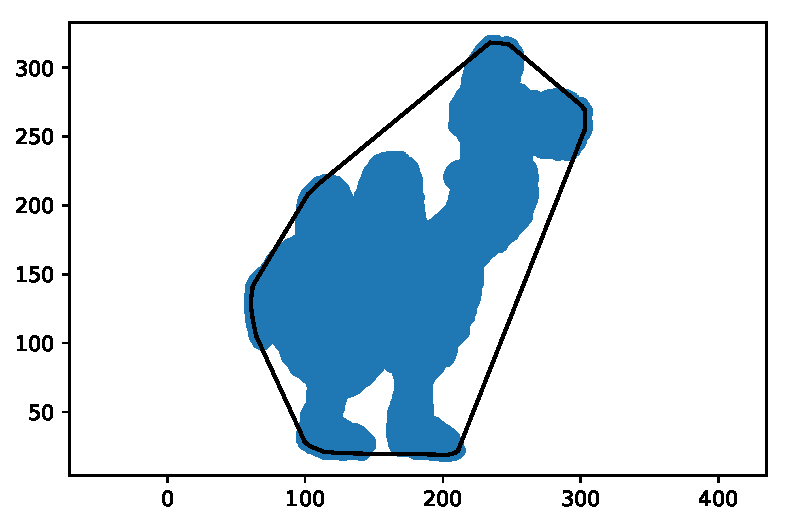
\includegraphics[width=.6\linewidth]{convhull.pdf}
 \caption{Convex hull of the image Camel.}
 \label{fig:tutorial:characterization:python:convhull}
\end{figure}

